\chapter{System Design\label{cha:design}}

As mentioned in Sec. \ref{sec:intro_strategy}, the overall target of this project is to develop four electronic modules and an electro-pneumatic actuation system for the 2010 Formula SAE vehicle. This chapter describes the design of these modules and the electro-pneumatic system, and provides context for design choices. The electrical portions of the design will be discussed in more detail than the mechanical portions, as the main focus of the thesis is electrical. 

Figure \ref{fig:design_overview} shows the electrical and mechanical interrelations between the 4 custom modules (in blue) and the systems they interact with. All of the modules communicate over a shared CANBus network, which eliminates point-to-point wiring between them.

\begin{figure}[H]
\centering
\begin{tikzpicture}[auto, node distance=2cm, draw=black!70, >=stealth']
  \node [bus] (bus1) {};
  \node [bus, below of=bus1] (bus2) {};
  \node [bus, below of=bus2, label={[rotate=-90]below:CAN Bus}] (bus3) {};

  \draw [-, line width=3pt] ($(bus1)+(0,1cm)$) -- (bus1) -- (bus2) -- (bus3) -- ++(0,-1cm);

  \node [block, right of=bus2, minimum width=2cm] (ecu) {ECU};
  \node [block, right of=ecu, font=\scriptsize, node distance=3cm] (engine) {Engine};
  \draw [<->, thick] (ecu) -- (bus2);
  \draw [<->, thick, dashed] (engine) -- (ecu);

  \node [block, blue shiny, right of=bus1, text width=1.7cm] (telemetry_module) {Telemetry Module};
  \node [block, right of=telemetry_module, text width=1.5cm, node distance=3cm] (dac) {DAQ};
  \draw [<->, thick] (telemetry_module) -- (bus1);
  \draw [<-, thick] (telemetry_module) -- (dac);
  \draw [->, thick] (ecu) -- (telemetry_module);
  \draw [-, thick] (telemetry_module.north) \antenna;

  \node [block, blue shiny, left of=bus1, text width=1.5cm] (brake_module) {Brake Module};
  \node [block, left of=brake_module, font=\scriptsize, text width=1.5cm, node distance=3cm] (brakes) {Braking System};
  \draw [<->, thick] (brake_module) -- (bus1);
  \draw [<->, thick, dashed] (brake_module) -- (brakes);
  
  \node [block, blue shiny, left of=bus2, text width=1.6cm] (engine_module) {Eng. \& Trans. Module};
  \node [block, left of=engine_module, font=\scriptsize, node distance=3cm] (intake) {Intake};
  \node [block, below of=engine_module, text width=2cm] (pneumatics) {Electro-pneumatics};
  \node [block, left of=pneumatics, font=\scriptsize, node distance=3cm] (transmission) {Transmission};
  \draw [<->, thick] (engine_module) -- (bus2);
  \draw [<->, thick, dashed] (engine_module) -- (intake);
  \draw [->, thick] (engine_module) -- (pneumatics);
  \draw [<->, thick, dashed] (pneumatics) -- (transmission);
  \draw [->, thick] (transmission) -- (engine_module);

  \node [block, blue shiny, right of=bus3, text width=1.6cm] (driver_interface) {Driver Interface Module};
  \node [block, right of=driver_interface, node distance=3cm, text width=1.25cm, font=\scriptsize] (controls) {Steering wheel controls};
  \draw [<->, thick] (driver_interface) -- (bus3);
  \draw [->, thick] (controls) -- (driver_interface);

  %%% Legend

  \draw [->, thick] ($(transmission.south west)+(0.5cm,-0.85cm)$) -- ++(0.5cm,0) node [label={[font=\tiny]below:Electrical}] {} -- ++(0.5cm,0);
  \draw [->, thick, dashed] ($(transmission.south west)+(2cm,-0.85cm)$) -- ++(0.5cm,0) node [label={[font=\tiny]below:Mechanical}] {} -- ++ (0.5cm,0);
  
\end{tikzpicture}

\caption{An overview of the interactions between the modules and the vehicle.}
\label{fig:design_overview}
\end{figure}

\section{Electro-Pneumatic System}

The electro-pneumatic system interfaces the engine and transmission module to the transmission's clutch and shift levers. The transmission controller portion of the engine and transmission module provide the control signals required to drive the electro-pneumatic system. The system design improves upon the previous generation discussed in Sec. \ref{sec:background_transmission} by targeting several of it's noted deficiencies while reusing aspects of the design that worked well.

A fully-electronic design was initially considered, but later abandoned. The finalized design calls for an improved valving scheme and a closed-loop feedback system. A thorough literature review was conducted to determine the best control system possible. 

The clutch actuation design incorporates a novel \emph{pulse-width modulation} (PWM) control scheme to allow for precise positioning control. The shift actuation design is unchanged from the previous implementation. 

\subsection{Fully-Electronic Consideration}

The possibility of using a fully electronic actuation system with geared DC motors was carefully considered. The control of such a system would be far simpler, as linear approximate models of DC motors are readily available. Reasonably priced gear-head motors from several suppliers were investigated. It was determined that any suitable fully-electronic system would be far heavier than it's pneumatic equivalent.

\subsection{Literature Review}

After deciding to keep a pneumatic actuation system, an improved valving scheme was proposed for the clutch, and sources of feedback were determined so that a closed-loop controller could be designed. Several academic papers were sourced that describe successful methods of pneumatic actuator control. \Citet{pneumatic_actuator} and \citet{adaptive_pneumatic} both use an electronically adjustable proportioning valve and a dual-acting cylinder. Proportioning valves are expensive (approximately \$300 from local suppliers) in comparison with binary solenoid valves (under \$50.)

Another approach by \citet{accurate_position} uses PWM signalled 3-way solenoid valves to control the air in and out of both sides of a dual-acting cylinder. By varying the duty cycle of the input signals, they were able to modulate the effective mass air flow rate through the cylinder ports: with the valve open, air would tend to flow from the high-pressure source into the cylinder, and with the valve closed, air would flow from the pressurized cylinder out through the exhaust port of the valve. This valving scheme allowed for a high degree of positional accuracy, however a large amount of air would be consumed during operation, as air is constantly being exhausted.

The dimensions of the pneumatic cylinders used in any implementation of this design are the same as those used in the previous designs. For this reason they will not be specified here.

\subsection{Mechanical Components}

A diagram of the mechanical portion of the pneumatics system is shown in Fig. \ref{fig:pneumatics_design}. As in the previous design, an on-board compressed air tank is fitted with a pressure regulator, which regulates the system pressure to approximately $\unit{0.8}{\mega\pascal}$. Four solenoid valves controlled with signals $U_U$, $U_D$, $U_A$, and $U_B$ control the flow of air to and from 2 pneumatic actuators.

\begin{figure}[H]
	\centering
	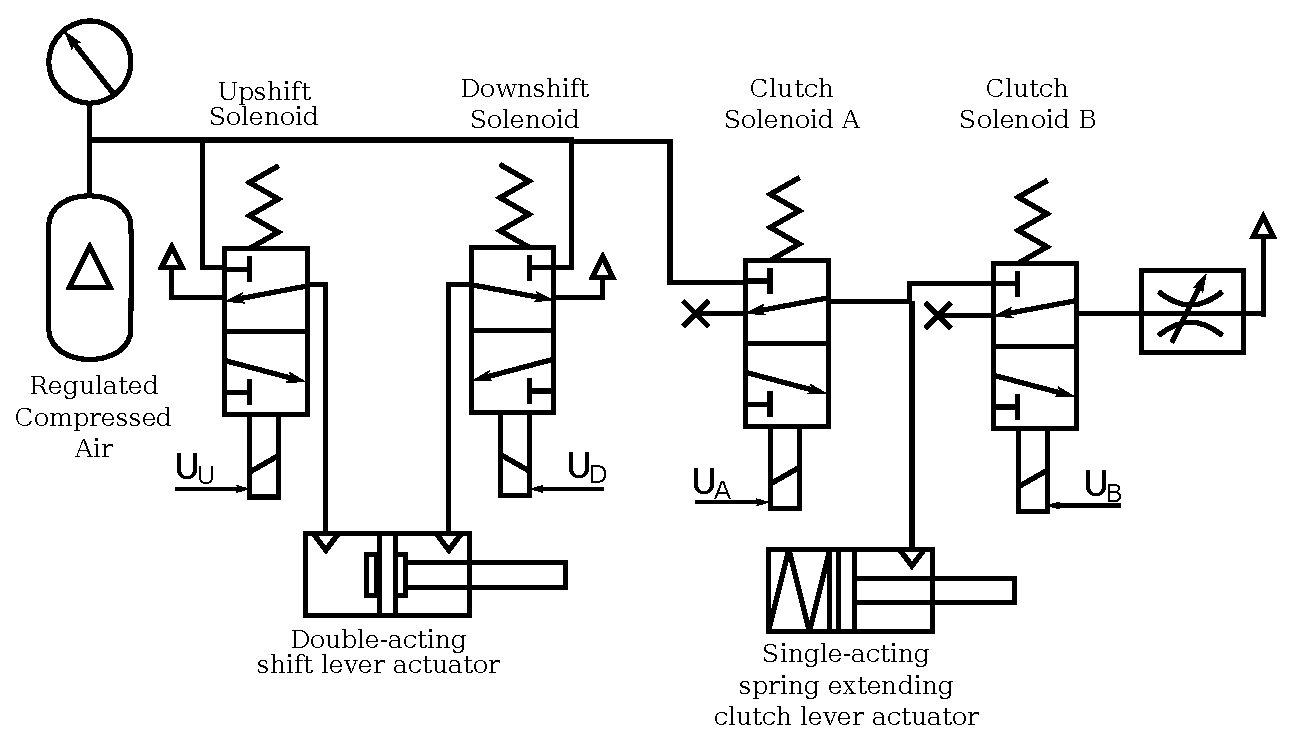
\includegraphics[scale=0.5]{design/figures/pneumatics}
	\caption{Transmission control pneumatics design.}
	\label{fig:pneumatics_design}
\end{figure}

\subsection{Clutch Lever Actuation}
\nomenclature{PWM}{Pulse Width Modulation}
\nomenclature{$U_U$, $U_D$}{Output signals from the transmission controller to the upshift and downshift solenoids.}
\nomenclature{$U_A$, $U_B$}{Pulse width modulated output signals from the transmission controller to clutch solenoids A and B.}

The three approaches described in \cite{pneumatic_actuator, adaptive_pneumatic, accurate_position} considered the possibility of a highly dynamic load on the actuator. The load seen by the clutch actuator is far more predictable than the loads they expected and is only uni-directional. Since the vehicle is only equipped with a limited supply of air, conservation is a concern. Taking these factors into account, a single-acting cylinder with a return spring is specified for the clutch, and we propose a new valving scheme that allows a degree of controllability over actuator while conserving as much air as possible.

The cylinder visible on the right of Fig. \ref{fig:pneumatics_design}, actuates the clutch lever. Precise control of the clutch is accomplished with fast solenoid valves \emph{Clutch Solenoid A} and \emph{Clutch Solenoid B}. These valves are signalled with \emph{pulse width modulated} (PWM) signals, which modulate the average mass air flow rate into and out separately of the cylinder. Positional feedback for the clutch cylinder is provided by a combination of an internal magnet on the piston in the cylinder and a magnetic sensing membrane potentiometer.

Both clutch solenoids are shown as 3-way (with exhaust ports) valves in Fig. \ref{fig:pneumatics_design}, but the valves are used in a 2-way configuration with the exhaust ports plugged.  This results in the following operation:

\begin{enumerate}
  \item When the pulse width modulated control signal $U_A$ to Clutch Solenoid A is non-zero, the valve will open, and air will flow into the cylinder at a rate proportional to the duty cycle, disengaging the clutch.
  \item When pulses no longer arrive at Clutch Solenoid A (or the duty cycle of $U_A$ approaches 0), the valve remains closed, and any air in the cylinder is trapped. The clutch maintains is position.
  \item When the pulse width modulated control signal $U_B$ to Clutch Solenoid B is non-zero, the valve will open, and any pressure differential between the cylinder and atmosphere will cause air to flow out of the cylinder to atmosphere at a rate proportional to the duty cycle. The clutch springs and the cylinders' internal spring work to return the actuator position to rest, and the clutch engages.
\end{enumerate}

An additional adjustable flow rate control valve (visible on the far right in Fig. \ref{fig:pneumatics_design}) was added to the design to allow additional tuning for during clutch engagement. The electro-pneumatic actuation system meets the controllability requirements outlined in \ref{sec:goals_transmission} when coupled with the transmission controller on the engine and transmission module. No air is wasted in disengaging the clutch and holding the position because the fill and exhaust operations are separately controlled with two valves.

\subsection{Shift Lever Actuation}

The shift lever does not require the same level of control as the clutch, and as such the design of the valving has not changed over previous implementations. Two binary valves are used with a dual-acting cylinder. The first actuator (visible on the left of Fig. \ref{fig:pneumatics_design}) actuates the shift lever between 3 different positions: up-shift, down-shift, and rest-state. The transmission spring-loads the lever to automatically return to the rest-state, which is half-way through the actuator stroke. Applying pressure to one port will pull the lever up, and applying pressure to the other port will pull the lever down.

Current gear position is determined with a potentiometer that is mechanically linked to the shift drum. Control and timing are generated by the engine and transmission controller.

\section{Engine and Transmission Module}

The engine and transmission module provides optimized selection of the variable-length intake, changes gears at the driver's request without requiring manual clutching, and provides transmission features that make driving easier. Figure \ref{fig:design_engine_overview} shows an overview of the engine and transmission module and it's interactions with the environment.

\begin{figure}[H]
	\centering
	\input{design/figures/engine_overview_block}
	\caption{An overview of the engine and transmission module and it's environmental interactions.}
	\label{fig:design_engine_overview_block}
\end{figure}

The intake runner position is mechanically actuated with a \emph{servo motor}. The module generates the control signals required by electro-pneumatic system to actuate both the clutch and shift levers. The ECU interfaces with the module both directly through discrete inputs and through the CAN bus.

\subsection{Processes}

The major processes of the engine and transmission module are \emph{up-shifting}, \emph{down-shifting}, and \emph{neutral find}. They are described at a high level using flow charts. Requests to perform these processes are broadcast over the network from the driver interface. The module listens for these requests and executes the correct process accordingly.

\subsubsection{Up-shifting}

The up-shift procedure is described in \ref{fig:transmission_upshift_flow}. Up-shifting does not require disengaging the clutch, merely a small decrease in engine RPM. The ECU provides a shift-cut feature to cut spark to the engine during a shift operation to avoid the driver having to manually modulate the throttle during a shift.

\begin{figure}[H]
	\centering
	\begin{tikzpicture}[auto, node distance=2cm, draw=black!70, >=stealth', font=\scriptsize]
  \node[start, text width=1.2cm] (start) {Upshift Request};
  \node [decision, right of=start, text width=1cm, inner sep=0pt, node distance=2.5cm] (at_top) {Top\\gear?};
  \node [end, below of=at_top] (done) {Done};
  \node [block, right of=at_top, text width=1.5cm, node distance=2.5cm] (shiftcut) {Enable shiftcut};

  \node [block, right of=shiftcut, text width=1.5cm, node distance=2.5cm] (wait_shiftcut) {Wait for RPM drop below $RPM^{TH}_{cut}$};
  \node [block, right of=wait_shiftcut, text width=1.5cm, node distance=2.5cm] (upshift) {Engage upshift solenoid};
  \node [block, right of=upshift, text width=1.5cm, node distance=2.5cm] (wait_upshift) {Wait for shift feedback};
  \node [block, below of=wait_upshift, text width=1.5cm] (upshift_off) {Disengage upshift solenoid};
  \node [block, left of=upshift_off, text width=1.5cm, node distance=2.5cm] (shiftcut_off) {Disable shiftcut};

  \draw [->, thick] (start) -- (at_top);
  \draw [->, thick] (at_top) -- node[]{yes} (done);
  \draw [->, thick] (at_top) -- node[]{no} (shiftcut);

  \draw [->, thick] (shiftcut) -- (wait_shiftcut);
  \draw [->, thick] (wait_shiftcut) -- (upshift);
  \draw [->, thick] (upshift) -- (wait_upshift);
  \draw [->, thick] (wait_upshift) -- (upshift_off);
  \draw [->, thick] (upshift_off) -- (shiftcut_off);
  \draw [->, thick] (shiftcut_off) -- (done);
\end{tikzpicture}

	\caption{Transmission upshift procedure.}
	\label{fig:transmission_upshift_flow}
\end{figure}

The up-shift process depends upon engine RPM and gear position, both of which are provided by the ECU. The shift-cut feature is engaged on the ECU to drop the engine RPM by a small amount known as the cut RPM threshold, or $RPM^{TH}_{cut}$. The exact value of $RPM^{TH}_{cut}$ can be tuned on the ECU. Once the RPM reaches the cut threshold, the upshift solenoid is engaged, which actuates the pneumatics to push the shift lever. Once the module receives notification that the current gear has incremented, the pneumatics are relaxed, and shift cut feature is disengaged.

\nomenclature{$RPM^{TH}_{cut}$}{The threshold RPM is expected to drop when shift-cut is engaged for no-lift up-shifting.}

\subsubsection{Down-shifting}

The down-shift procedure is described in \ref{fig:transmission_downshift_flow}. Unlike up-shifting, down-shifting requires disengaging the clutch, merely a small decrease in engine RPM. The ECU provides a shift-cut feature to cut spark to the engine during a shift operation to avoid the driver having to manually modulate the throttle during a shift.

When the Transmission Manager receives a down-shift request over the network, similar to the up-shift request handling, it creates asynchronous events in the Event Scheduler to respond to the request. Figure \ref{fig:transmission_downshift_flow} shows the flow chart of the downshift procedure. Clutch engagement and disengagement is handled asynchronously by the Clutch Controller. The downshift procedure differs from the upshift procedure in that the downshift requires use of the clutch, as well as two asynchronous incoming events from the driver:

\begin{enumerate}
  \item The original downshift request, when the driver pulls and holds the downshift paddle on the steering wheel, and
  \item a clutch engagement request, issued when the driver releases the downshift paddle.
\end{enumerate}

Adding this extra clutch engagement request allows the driver to delay re-engagement of the clutch so that they can blip the throttle to avoid engine compression and the possibility of a spinout when the clutch plates re-engage (this was explained in Sec. \ref{sec:background_transmission}.)

Additionally, a minimum clutch disengagement time $t^{clutch}_{min}$ is observed (another tunable parameter) in the event the driver pulls the paddle and releases it without any delay.

\nomenclature{$t^{clutch}_{min}$}{Minimum clutch disengagement time during a downshift request.}

\begin{figure}[H]
\centering
\begin{tikzpicture}[auto, node distance=2cm, draw=black!70, >=stealth', font=\scriptsize]
  \node[start, text width=1.4cm] (start) {Downshift Request};
  \node [decision, right of=start, text width=1cm, inner sep=0pt, node distance=2.5cm] (in_neutral) {Neutral?};
  \node [end, below of=in_neutral] (done) {Done};
  \node [block, right of=in_neutral, text width=1.5cm, node distance=2.5cm] (clutchin) {Disengage clutch};

  \node [block, right of=clutchin, text width=1.5cm, node distance=2.5cm] (downshift) {Engage downshift solenoid};
  \node [block, right of=downshift, text width=1.5cm, node distance=2.5cm] (wait_downshift) {Wait for shift feedback};
  \node [block, right of=wait_downshift, text width=1.5cm, node distance=2.5cm] (downshift_off) {Disengage downshift solenoid};
  \node [block, below of=downshift_off, text width=1.5cm] (wait_clutchin) {Wait for clutch-in request};
  \node [block, left of=wait_clutchin, text width=1.5cm, node distance=2.5cm] (clutchout) {Engage clutch};

  \draw [->, thick] (start) -- (in_neutral);
  \draw [->, thick] (in_neutral) -- node[]{yes} (done);
  \draw [->, thick] (in_neutral) -- node[]{no} (clutchin);

  \draw [->, thick] (clutchin) -- (downshift);
  \draw [->, thick] (downshift) -- (wait_downshift);
  \draw [->, thick] (wait_downshift) -- (downshift_off);
  \draw [->, thick] (downshift_off) -- (wait_clutchin);
  \draw [->, thick] (wait_clutchin) -- (clutchout);

  \draw [->, thick] (clutchout) -- (done);
\end{tikzpicture}

\caption{Transmission downshift procedure.}
\label{fig:transmission_downshift_flow}
\end{figure}

\subsubsection{Variable Intake}

\subsubsection{Gear Selection \label{sec:design_engine_transmission_gear_selection}}


\subsubsection{Advanced Transmission Features}

\begin{description}

\item[Auto Upshift Feature]

This feature of the engine module is aimed primarily at improving performance in the acceleration event. Based on known torque curves, a table of optimal shift points in the RPM range is developed. As the engine reaches the top RPM for a given gear, the engine module will automatically upshift to the next gear, without any driver input. All the driver needs to do is maintain full throttle, and hold on.

\item[Launch]
Full-throttle launch uses an important feature of the ECU called launch control. From a stand-still, the slip ratio of the driven wheels to the non-driven wheels is monitored, and the engine output power is reduced until the ratio reaches 1:1. Drivers use this feature by maintaining full-throttle at the starting line while holding the brake pedal. As soon as the brake pedal is released, the the engine module will release the clutch in a controlled manner in an attempt to get the best possible acceleration.

\item[Crawl]
Part-throttle launch is a feature designed to mimic an automatic transmission. By controlling the clutch position, and thereby modulating the amount of torque transferred to the wheels for a short period of time, the car can be made to creep slowly from a standstill. This will be used when driving up to the starting line of various dynamic events.

\item[Neutral Find]
As drivers come in to the pits from driving the course, a useful feature is the ability for the car to shift the transmission back into neutral to avoid stalling the car. The neutral find feature will automatically downshift the transmission repeatedly until it finds neutral.

\end{description}


\subsection{Software}

Software overview diagram


\subsubsection{Transmission Manager}

Listens to transmission requests from the driver over the network.

Uses the event scheduler to sequence the complex series of actuation vectors required by upshifting and downshifting.

Implement the PID feedback controller used to actuate the pneumatic system.

Interacts with the PWM generator to create the control signals required to actuate the pneumatic system.


\subsubsection{Intake Manager}

Continously monitor engine RPM and throttle position through messages from the ECU.

Will adjust intake runner length based on a functional map of RPM and throttle position.

Use hysterisis to avoid instability.

Map will be generated through dynometer testing.


\subsubsection{Starter Manager}

Listen for driver requests to start the engine.

Provide a means of one-touch starting -- sequences the actual starting of the engine through the solenoid driver. 


\subsubsection{Event Scheduler}

Allow for complex sequencing of events in time.

Controllers may schedule new events to occur at various points in time.

Scheduler will continuously update the schedule and signal the main control loop to execute events that are now current.


\subsubsection{CAN Interface}

Provide a means of interfacing with the physical bus. 

Allow direction of particular messages to particular modules.


\subsubsection{PWM Generator}

Generate PWM signals of at least 20 Hz with a resolution of 1\% duty
cycle.

Two-channel design


\subsubsection{Main Control Loop}

Initializes the system and brings into a known state.

Waits for pending events to be executed and executes them.

Monitor for system faults and react accordingly.


\subsection{Hardware}

Show system hardware diagram


\subsubsection{Microcontroller}

Execute system control software.

In-circuit programmable and debuggable.

Has built-in CAN controller.

Has built-in RAM and ROM as well as EEPROM for holding configuration parameters.


\subsubsection{CAN transceiver}

Interface module with the CAN bus.

Be capable of terminating the bus.


\subsubsection{High current solenoid drivers}


Controlling pneumatic solenoid valves (4)

Controlling starter solenoid


\subsubsection{I/O lines to the ECU}

The engine and transmission module has a several CMOS-level outputs to discrete control pins on the ECU:

\begin{itemize}
  \item A line to the launch control pin, which when toggled enables and disables the launch control feature,
  \item A line to the shift cut pin, which when held high enables shift cut, decreasing engine power to allow for an upshift,
  \item A line to the traction cut percent pin, which is a \unit{0-5}{\volt} level signalled input changing the amount of acceptable wheel slip before traction control cuts in.
  \item A line to the traction control on/off pin, which toggles the traction control feature,
  \item A line to the traction control wet/dry pin, which swaps between two traction control presets.
\end{itemize}

The outputs of these lines are controlled in the system software through the event scheduler. 
\section{Braking Module\label{sec:Braking-Module-Design}}

The braking module adjusts the brake bias electronically as requested by the driver. It also provides the ability to calibrate itself to account for mechanical wear and a degree of component tolerance that may cause unwanted rotation of the balance bar. Figure \ref{fig:design_brake_overview_block} shows an overview of the braking module and it's interactions with the environment. 

\begin{figure}[H]
\centering
\begin{tikzpicture}[auto, node distance=2cm, draw=black!70, >=stealth', font=\footnotesize]
  \node [block, minimum width=2cm, inner xsep=0] (pressure1) {Front Pressure Sensor};
  \node [block, minimum width=2cm, inner xsep=0, right of=pressure1, node distance=4cm] (pressure2) {Front Pressure Sensor};

  \node [block, blue shiny, minimum width=6cm, text width=4cm, below of=pressure1, right=-1cm, node distance=1.5cm] (module) {Braking Module};

  \node [block, below of=pressure1, right=-1cm, node distance=3cm, text width=1.1cm] (eot1) {Left EOT Switch};
  \node [block, below of=pressure2, left=-1cm, node distance=3cm, text width=1.1cm] (eot2) {Right EOT Switch};

  \node at ($(eot1)!0.5!(eot2)$) [red shiny, circle, label={[text width=1.5cm, rotate=90, below=5pt, left=10pt]below right:Stepper Motor}] (motor) {M};

  \node [rectangle, below of=motor, minimum width=2cm, label=below:Bias Bar, pattern=north east lines, node distance=1cm] (bias) {};

  \draw [->, thick] (pressure1.south) to ($(module.north west)!(pressure1.south)!(module.north east)$);
  \draw [->, thick] (pressure2.south) to ($(module.north west)!(pressure2.south)!(module.north east)$);

  \draw [->, thick] (eot1.north) to ($(module.south west)!(eot1.north)!(module.south east)$);
  \draw [->, thick] (eot2.north) to ($(module.south west)!(eot2.north)!(module.south east)$);

  \draw [<-, thick] (motor.north) to ($(module.south west)!(motor.north)!(module.south east)$);
  \draw [->, thick, dashed] (motor.south) to ($(bias.north west)!(motor.south)!(bias.north east)$);

  \draw [->, thick, dashed] (bias) -| (eot1);
  \draw [->, thick, dashed] (bias) -| (eot2);

  %%% CAN Bus

  \node [bus, name=can1, right of=module, label={[rotate=90, left=0.75cm]below right:CAN Bus}, node distance=3.5cm] {CAN Bus};
  \node [bus, name=can2, below of=can1, node distance=1cm] {};
  \node [bus, name=can3, above of=can1, node distance=1cm] {};

  \draw [<->, thick] (module) to (can1);
  \draw [-, line width=3pt] (can1) -- (can2);
  \draw [-, line width=3pt] (can1) -- (can3);

  %%% Legend

  \draw [->, thick] ($(eot2.east)+(2cm,0cm)$) -- ++(0.5cm,0) node [label={[font=\tiny]below:Electrical}] {} -- ++(0.5cm,0);
  \draw [->, thick, dashed] ($(eot2.south east)+(2cm,0cm)$) -- ++(0.5cm,0) node [label={[font=\tiny]below:Mechanical}] {} -- ++ (0.5cm,0);
\end{tikzpicture}
\caption{Overview of the braking module and it's environment.}
\label{fig:design_brake_overview_block}
\end{figure}

A \emph{stepper motor} is connected to the balance bar and used to rotate it to the desired position. The motor is bi-directional and can provide the resolution required to allow a 0.5\% bias ratio adjustment. Two \emph{end-of-travel switches} are used to determine when the balance bar is at it's end of travel. \emph{Pressure sensors} on the front and rear braking cylinders are used to determine the current pressure in each system. These components were chosen as part of the mechanical design of the brake pedal assembly by another team member. The actual choice of stepper motor has yet to be determined.

\subsection{Driver-Initiated Processes \label{sec:braking_processes}}

The major processes of the braking module are \emph{brake bias adjustment}, \emph{brake bias calibration}, and \emph{pressure calibration}. Requests to perform either of the processes are broadcast over the network from the driver interface. The module listens for these requests and executes the correct process accordingly. 

\subsubsection{Brake Bias Adjustment}

The brake bias adjustment procedure is shown in Fig. \ref{fig:design-braking-bias-adjustment}. The module performs a series of safety checks before rotating the balance bar to adjust the relative force distribution between the two brake master cylinders.

\begin{figure}[H]
	\centering
	\begin{tikzpicture}[auto, node distance=2cm, draw=black!70, >=stealth', font=\scriptsize]
  \node [start] (start) {Start};
  \node [decision, right of=start, text width=1cm, inner sep=0pt] (brakes_on) {Safe to\\adjust?};
  \node [decision, right of=brakes_on, text width=1cm, inner sep=0pt, node distance=2.5cm] (valid_bias) {Valid bias?};
  \node [end, below of=start, node distance=1cm] (abort) {Abort};

  \node [block, right of=valid_bias, text width=1.5cm, inner xsep=0pt, node distance=2.5cm] (calc) {Calculate offset steps};
  \node [block, right of=calc, text width=1.5cm, inner xsep=0pt, node distance=2.5cm] (step) {Step by offset};
  \node [block, right of=step, text width=1cm, inner xsep=0pt] (store) {Store new offset};
  \node [end, right of=store] (done) {Done};

  \draw [->, thick] (start) to (brakes_on);
  \draw [->, thick] (brakes_on) to (valid_bias);
  \draw [->, thick] (brakes_on.south) |- node[below]{yes} (abort);
  \draw [->, thick] (valid_bias.south) |- node[below]{no} (abort);
  \draw [->, thick] (brakes_on) to node[above]{no} (valid_bias);
  \draw [->, thick] (valid_bias) to node[above]{yes} (calc);
  \draw [->, thick] (calc) to (step);
  \draw [->, thick] (step) to (store);
  \draw [->, thick] (store) to (done);
\end{tikzpicture}

	\caption{Flow-chart for the brake bias adjustment procedure.}
	\label{fig:design-braking-bias-adjustment}
\end{figure}

Of prime importance is that the vehicle is not in motion and the brakes are not engaged while the adjustment is underway. The desired bias ratio is also validated before any adjustment is attempted. If the vehicle is stopped, the brakes are not engaged, and the request is valid, the adjustment may proceed. The module calculates the number of steps required to move from the current position to the desired offset and signals the motor to advance this many steps in the correct direction.

\subsubsection{Brake Bias Calibration}

A flow-chart of the brake bias calibration procedure is shown in Fig. \ref{fig:brake_bias_calibration_flow}. By recording the number of steps it takes to rotate the balance bar from through it's range of motion, we can determine the correct centre point for the bias bar. 

\begin{figure}[H]
	\centering
	\begin{tikzpicture}[auto, node distance=2cm, draw=black!70, >=stealth', font=\scriptsize]
  \node [start] (start) {Start};

  \node [block, right of=start, text width=1cm, inner xsep=0pt] (step_left) {Step Left};
  \node [decision, right of=step_left, text width=1.0cm, inner sep=0pt] (at_left) {At leftend?};

  \node [block, right of=at_left, text width=1cm, inner xsep=0pt] (step_right) {Step Right};
  \node [block, right of=step_right, text width=1cm, inner xsep=2pt] (count) {Add to count};
  \node [decision, right of=count, text width=1cm, inner sep=0pt] (at_right) {At rightend?};

  \node [block, below of=at_right, text width=2cm, inner xsep=2pt, node distance=2.5cm] (adjust) {Adjust bias to old value};
  \node [block, left of=adjust, text width=1.5cm, inner xsep=2pt, node distance=3cm] (store) {Store calibration};
  \node [end, left of=store, node distance=7cm] (end) {Done};

  \draw [->, thick] (start) to node[coordinate, name=x1]{} (step_left);
  \draw [->, thick] (step_left) to (at_left);
  \draw [->, thick] (at_left.south) -- ++(0,-0.25) node[below]{no} -| (x1);
  \draw [->, thick] (at_left.east) to node[name=x2]{yes} (step_right);
  \draw [->, thick] (step_right) to (count);
  \draw [->, thick] (count) to (at_right);
  \draw [->, thick] (at_right.south) -- ++(0,-0.25) node[below]{no} -| (x2);

  \draw [->, thick] (at_right.east) -- ++(0.5,0) node[above]{yes} |- (adjust);
  \draw [->, thick] (adjust) to (store);
  \draw [->, thick] (store) to (end);
\end{tikzpicture}

	\caption{Flow-chart for the brake bias calibration procedure.}
	\label{fig:brake_bias_calibration_flow}
\end{figure}

The first step in calibrating the brake bias is to rotate the balance bar to it's leftmost point of travel, where it pushes on the left end-of-travel switch. This signals the module that the leftmost extreme has been reached. Next, the balance bar is rotated to it's rightmost point of travel, until it pushes on the right end-of-travel switch. The module counts the steps required to travel through it's range of motion and saves the count in non-volatile parameter storage. Finally, the brake bias ratio is adjusted back to it's previous value.

\subsubsection{Pressure Calibration}

The pressure sensor calibration routine is outlined in Fig. \ref{fig:brake_pressure_calibration_flow}. The module keeps track of the minimum and maximum pressures that will be present in both the front and rear systems. This allows it to determine when the brakes are engaged, and to what extent.

\begin{figure}[H]
	\centering
	\begin{tikzpicture}[auto, node distance=2cm, draw=black!70, >=stealth', font=\scriptsize]
  \node [start] (start) {Start};
  \node [decision, right of=start, right=0cm, text width=1.4cm, inner sep=0pt] (min) {Min Applied?};
  \node [block, right of=min, text width=2cm, inner xsep=0pt, node distance=3cm] (sample1) {Sample Pressures};
  \node [decision, right of=sample1, right=0cm, text width=1.4cm, inner sep=0pt] (max) {Max Applied?};
  \node [block, right of=max, text width=2cm, inner xsep=0pt, node distance=3cm] (sample2) {Sample Pressures};

  \node [decision, below of=sample2, text width=1.4cm, inner sep=0pt, node distance=2.5cm] (valid) {Valid samples?};
  \node [block, left of=valid, text width=1.5cm, inner xsep=2pt, node distance=3cm] (save) {Save Calibration};

  \node [end, below of=save] (success) {Success};
  \node [end, below of=valid] (fail) {Fail};

  \draw [->, thick] (start) -- ($(start.east)!0.5!(min.west)$) node[name=x1,coordinate]{} -- (min);
  \draw [->, thick] (min.south) -- ++(0,-0.25cm) node[below]{no} -| (x1);
  \draw [->, thick] (min) to node [] {yes} (sample1);

  \draw [->, thick] (sample1) to node [name=x2]{} (max);
  \draw [->, thick] (max.south) -- ++(0,-0.25cm) node[below]{no} -| (x2);
  \draw [->, thick] (max) to node [] {yes} (sample2);

  \draw [->, thick] (sample2) to (valid);
  \draw [->, thick] (valid) to node [above] {yes} (save);

  \draw [->, thick] (save) to (success);
  \draw [->, thick] (valid.south) to node [] {no} (fail);

\end{tikzpicture}
	\caption{Flow-chart for the brake pressure calibration sequence.}
	\label{fig:brake_pressure_calibration_flow}
\end{figure}

The first step of pressure calibration is to ask the driver to apply minimum pressure. The brake module signals the driver interface to request the driver take their foot off the brake. Once done, the driver interface signals the brake module that minimum pressure has been applied. The brake module then samples the current pressure in both systems. This procedure is repeated for maximum pressure by asking the driver to push on the brake as hard as possible. If the samples are valid, meaning the minimum pressures are less than the maximum pressures and there is a minimum pressure difference between fully-released and fully-applied, the sampled pressures are stored in non-volatile memory.

\subsection{Hardware}

A high-level overview of the module's hardware design is shown in Fig. \ref{fig:brake_hardware_design_block}. Like the other modules, the heart of the brake module is a micro-controller that runs the software necessary to implement all of the required features. 

\begin{figure}[H]
\centering
\begin{tikzpicture}[auto, node distance=2cm, draw=black!70, >=stealth']
%  \draw[help lines] (-3,-5) grid (8,2);

  %%% Pressure Sensors
  \node [block, name=pressure1, font=\scriptsize, text width=1.5cm, inner xsep=0] {Front Pressure Sensor};
  \node [block, name=pressure2, right of=pressure1, font=\scriptsize, text width=1.5cm, inner xsep=0] {Rear Pressure Sensor};

  %%% Balance bar and EOT switches
  \node [block, name=eot1, right of=pressure2, font=\scriptsize, text width=1.5cm, node distance=3cm] {Left EOT Switch};
  \node [block, name=balance, right of=eot1, font=\scriptsize, text width=1.25cm, inner xsep=0] {Balance Bar};
  \node [block, name=eot2, right of=balance, font=\scriptsize, text width=1.5cm] {Right EOT Switch};

  \node [red shiny, circle, below of=balance, name=motor, node distance=1cm, inner sep=1pt] {M};
  \node [block, below of=motor, node distance=1cm, text width=1.5cm, font=\scriptsize] (driver) {Stepper Driver};

  \draw [->, dashed, thick] (balance) -- (eot1);
  \draw [->, dashed, thick] (balance) -- (eot2);
  \draw [->, dashed, thick] (motor) -- (balance);
  \draw [->, thick] (driver) -- (motor);

  \node [block, name=adc1, below of=pressure1, text width=1.5cm] {ADC};
  \node [block, name=adc2, below of=pressure2, text width=1.5cm] {ADC};

  %%% Microcontroller block
  \path ($(adc1.south west)+(0,-1cm)$) node (mu1) {};
  \path ($(adc1.south west -| eot2.south east) + (0,-1cm)$) node (mu2) {};

  \node [block, name=micro, fit=(mu1) (mu2), inner xsep=0, minimum height=1cm] {Microcontroller};

  \draw [->, thick] (pressure1) to (adc1);
  \draw [->, thick] (pressure2) to (adc2);
  \draw [->, thick] (adc1.south) -- ($(micro.north west)!(adc1.south)!(micro.north east)$);
  \draw [->, thick] (adc2.south) -- ($(micro.north west)!(adc2.south)!(micro.north east)$);

  \draw [->, thick] (eot1.south) -- ($(micro.north west)!(eot1.south)!(micro.north east)$);
  \draw [->, thick] (eot2.south) -- ($(micro.north west)!(eot2.south)!(micro.north east)$);

  \draw [<-, thick] (driver.south) -- ($(micro.north west)!(driver.south)!(micro.north east)$);

  %%% CAN Bus

  \node at ($(micro.east)+(2cm,0)$) [block, name=can, node distance=2cm, inner xsep=2pt] {CAN Transceiver};

  \draw [<->, thick] (micro) to (can);

  \node [bus, name=can1, above of=can, label=above:CAN Bus, node distance=2.5cm] {CAN Bus};
  \node [bus, name=can2, left of=can1, node distance=1cm] {};
  \node [bus, name=can3, right of=can1, node distance=1cm] {};

  \draw [-, line width=3pt] (can) -- (can1);
  \draw [-, line width=3pt] (can1) -- (can2);
  \draw [-, line width=3pt] (can1) -- (can3);

  %%% Background

  \begin{pgfonlayer}{background}
    \path (adc1.north west)+(-0.3,0.3) node (a) {};
    \path (can.south east)+(+0.2,-0.2) node (b) {};
    \path[module] (a) rectangle (b);
  \end{pgfonlayer}

  %%% Legend

  \draw [->, thick] ($(micro.south west)+(0.5cm,-0.5cm)$) -- ++(0.5cm,0) node [label={[font=\tiny]below:Electrical}] {} -- ++(0.5cm,0);
  \draw [->, thick, dashed] ($(micro.south west)+(2cm,-0.5cm)$) -- ++(0.5cm,0) node [label={[font=\tiny]below:Mechanical}] {} -- ++ (0.5cm,0);
\end{tikzpicture}

\caption{Block diagram of the braking module hardware.}
\label{fig:brake_hardware_design_block}
\end{figure}

The module communicates over the bus using a CAN transceiver. A pair of analog-to-digital converters (similar to those used in the engine and transmission module) sample the brake pressure sensors. Unique to the brake module is a \emph{stepper motor driver} that provides the signals necessary to drive the stepper motor connected to the balance bar. The micro-controller interfaces to the end-of-travel switches without any extra hardware.

\subsubsection{Stepper Motor Driver}

The stepper motor driver generates the signals required to drive the stepper motor connected to the balance bar. It must be capable of  driving a bi-polar stepper motor in the clockwise or counter-clockwise direction. It must also supply enough current to generate the torque required to spin the balance bar, which is approximately\footnote{This figure was supplied by the team member responsible for the braking pedal assembly.} \unit{150}{mA}.

\subsubsection{Analogue-to-Digital Converters (ADC)}

The ADCs sample the output voltage from pressure sensors attached to the front and rear brake master cylinders. The output voltage of the particular sensors used is \unit{0-5}{\volt}, corresponding to \unit{0-10}{\mega\pascal}. The expected maximum brake pressure is somewhere around \unit{7}{\mega\pascal}. To achieve resolution of \unit{10}{\kilo\pascal}, a 10-bit ADC is sufficient. The pressure values are sampled at \unit{10}{\hertz}.

\subsubsection{End-of-Travel Sensing Switches}

Two end-of-travel switches are tripped whenever the balance bar reaches it's leftmost or rightmost extremes. The switches are normally high-impedance, and become switched to ground. The micro-controller should have GPIO pins with weak internal pull-up resistors to detect the state of the switches.

\subsection{Software}

A block-diagram overview of the software design is shown in Fig. \ref{fig:brake_software_design_block}. The functionality of the system is separated into a \emph{bias manager} and a \emph{pressure manager}. Like the engine and transmission module, the managers interact with a set of hardware abstraction interfaces to perform their tasks, and the entire process is overseen by a \emph{module coordinator}.

\begin{figure}[H]
	\centering
	\tikzstyle{big arrow} = [>=latex, line width=4pt, gray]

\begin{tikzpicture}[auto, node distance=2cm, draw=black!70, >=stealth']
  \node [block, minimum width=2cm, inner xsep=0] (stepper) {Stepper Interface};
  \node [block, minimum width=2cm, inner xsep=0, right of=stepper, node distance=3cm] (io) {I/O Interface};

  \node [block, grey shiny, minimum width=5cm, inner xsep=0, below of=stepper, right=-1cm, text width=5cm, node distance=2cm] (bias_manager) {Bias Manager};

  \node [block, minimum width=2cm, inner xsep=0, below of=stepper, node distance=4cm] (can) {CAN Interface};
  \node [block, minimum width=2.2cm, inner xsep=0, below of=io, node distance=4cm] (nv) {NV Storage Interface};
  \node [block, blue shiny, minimum width=2.5cm, text width=2.2cm, inner xsep=0, right of=nv, node distance=3cm] (coordinator) {Module Coordinator};
  \node [block, minimum width=2cm, inner xsep=0, left of=can, node distance=3cm] (adc) {ADC Interface};

  \node [block, grey shiny, minimum width=5cm, inner xsep=0, below of=can, right=-1cm, text width=5cm, node distance=2cm] (pressure_manager) {Pressure Manager};

  \draw [<-, big arrow] (stepper.south) -- ($(bias_manager.north west)!(stepper.south)!(bias_manager.north east)$);
  \draw [->, big arrow] (io.south) -- ($(bias_manager.north west)!(io.south)!(bias_manager.north east)$);

  \draw [<->, big arrow] (can.north) -- ($(bias_manager.south west)!(can.north)!(bias_manager.south east)$);
  \draw [<->, big arrow] (nv.north) -- ($(bias_manager.south west)!(nv.north)!(bias_manager.south east)$);

  \draw [<->, big arrow] (can.south) -- ($(pressure_manager.north west)!(can.south)!(pressure_manager.north east)$);
  \draw [<->, big arrow] (nv.south) -- ($(pressure_manager.north west)!(nv.south)!(pressure_manager.north east)$);

  \draw [<->, big arrow] (bias_manager) -| (coordinator);
  \draw [<->, big arrow] (pressure_manager) -| (coordinator);
  \draw [->, big arrow] (adc) |- (pressure_manager);

  \draw [-, thick] ($(coordinator.south)!0.5!(coordinator.south west)$) |- ($(nv.south)!0.5!(nv.south east)+(0,-0.6cm)$) node [name=x, inner sep=0]{};
  \draw [->, thick] (x) -- ($(nv.south)!0.5!(nv.south east)$);
  \draw [->, thick] (x) -| ($(can.south)!0.5!(can.south east)$);

  \draw [-, thick] (adc.east) -| ($(stepper.south west)+(-0.5cm,-0.6cm)$) node [name=x2, inner sep=0]{};
  \draw [->, thick] (x2) -| ($(stepper.south)!0.5!(stepper.south east)$);
  \draw [->, thick] (x2) -| ($(io.south)!0.5!(io.south east)$);
  
\end{tikzpicture}

	\caption{Block diagram of the braking module software.}
	\label{fig:brake_software_design_block}
\end{figure}

Several hardware abstraction interfaces link the external hardware and micro-controller features to the bias and pressure managers. Unique to the braking module is the \emph{stepper motor interface}. The CAN interface is exactly as described earlier, and is not mentioned here.

\subsubsection{Bias Manager}

The bias manager implements the bias adjustment and bias calibration processes. It listens for requests to initiate either process from the network by way of the CAN interface.

When asked to adjust the brake bias, the bias manager coordinates with the pressure manager to determine if the brakes are being applied, and with the engine and transmission controller to determine if the vehicle is in motion. It performs the calculations required to calculate the new bias position, and adjusts the balance bar accordingly by sending motor step commands to the stepper motor interface.

Bias calibration requires similar coordination to ensure a safe operating state. The bias manager again uses the stepper motor interface to move the balance bar between it's extremes. Calibration data is loaded at start-up and stored after calibration in NVRAM by way of the non-volatile storage interface.

\subsubsection{Pressure Manager}

The pressure manager periodically outputs the front and rear brake pressures. It also implements the pressure calibration procedure and listens for calibration requests over the network, similar to the bias manager.

The front and rear pressures are sampled through the ADC interface. The pressure manager uses the CAN interface to output the samples over the network. Current pressure readings are made available to the bias manager to avoid adjusting or calibrating the bias while the brakes are engaged.

The pressure manager communicates with the driver interface through the CAN interface to coordinate the sequence of driver inputs required to calibrate the front and rear brake pressures. Like the pressure manager, calibration data is loaded at start-up and stored after calibration through the non-volatile storage interface.

\subsubsection{Module Coordinator}

Like the module coordinator for the engine and transmission module, the braking module coordinator contains the low-level state machine mechanisms needed by the two managers to transition between their internal states. It keeps track of the current state of the system, and also initializes all of the hardware abstraction interfaces and managers at start-up time. 

\subsubsection{Stepper Motor Interface}

The stepper motor interface takes motor movement commands from the program and converts them into commands for the stepper motor driver. It can direct the stepper motor driver to turn clockwise or counter-clockwise, and move an arbitrary number of steps. 

\subsubsection{GPIO Interface}

The GPIO interface monitors the state of the end-of-travel buttons. It can asynchronously interrupt the program when a change of state occurs. 

\subsubsection{ADC Interface}  

The ADC interface initiates a sampling cycle on either pressure sensor channel. The resulting sample is provided to  the program for further processing. 

\subsubsection{Non-Volatile Storage Interface}

The \emph{non-volatile storage interface} reads and writes calibration data to the non-volatile storage portion of the micro-controller. It is also used to keep track of the current position of the bias bar, so calibration is not required between start-ups.


\section{Telemetry Module\label{sec:Telemetry-Module-Design}}

The \emph{telemetry module} provides a means for multiplexing the ECU and DAQ data streams, and sending them wirelessly to the crew's laptops. The module also decodes data from the DAQ and makes it available over the network to other modules, and injects data from other modules into the DAQ stream. An overview of the telemetry module and its environmental interactions is shown in Fig.\ \ref{fig:design_telemetry_overview_block}.

\begin{figure}[H]
	\centering
	\begin{tikzpicture}[auto, node distance=2cm, draw=black!70, >=stealth']
  \node [block, blue shiny, minimum width=4cm, text width=4cm] (module) {Telemetry Module};
  \node [block, left of=module, node distance=4cm, font=\scriptsize, text width=1.5cm] (modem) {Wireless Modem};
  \node [block, below of=module, left=-2cm, text width=1cm, node distance=1.5cm] (ecu) {ECU};
  \node [block, below of=module, right=-2cm, text width=1cm, node distance=1.5cm] (dac) {DAC};

  \draw [-, thick] (modem.north) \antenna;
  \draw [<->, thick] (modem) -- (module);
  \draw [<->, thick] (ecu) -- ($(module.south west)!(ecu.north)!(module.south east)$);
  \draw [<->, thick] (dac) -- ($(module.south west)!(dac.north)!(module.south east)$);

  \node [bus, right of=ecu] (can1) {};
  \node [bus, above of=can1, node distance=1.5cm] (can2) {};

  \draw [-, line width=3pt] (can1) -- ++(0,-1cm);
  \draw [-, line width=3pt] (can1) -- node[label={[rotate=90]below:CAN Bus}]{} (can2) -- ++(0,1cm);
  \draw [<->, thick] (ecu) -- (can1);
  \draw [<->, thick] (module) -- (can2);
\end{tikzpicture}

	\caption{Overview of the telemetry module and it's environment.}
	\label{fig:design_telemetry_overview_block}
\end{figure}

The vehicle-side of the telemetry system consists of the telemetry module itself, which gathers and multiplexes the data from the ECU and DAQ over their serial links, and the \emph{wireless modem}, which transmits and receives data wirelessly from the remote laptops. The remote-side of the telemetry system consists of an off-the-shelf wireless receiver, which receives the data and makes it available on an RS-232 port on the laptop.

\subsection{ECU Data Channel}

The ECU data channel is illustrated in Fig.\ \ref{fig:ecu_data_channel}. It is a simple bi-directional pass-through channel. The module acts as a router for ECU data. The data stream is not modified in any way. 

\begin{figure}[H]
	\centering
	\begin{tikzpicture}[auto, node distance=2cm, draw=black!70, >=stealth', font=\scriptsize, minimum height=1cm]
  \node [block, text width=1cm] (ecu) {ECU};
  \node [block, right of=ecu, text width=1cm] (packetizer) {MUX};
  \node [block, right of=packetizer, text width=1.25cm] (modem1) {Wireless Modem};
  
  \draw [->, thick] (ecu) -- (packetizer);
  \draw [->, thick] (packetizer) -- (modem1);
  \draw [-, thick] (modem1.east) -- ++(0.5cm,0) \antenna;

  \node [block, right of=modem1, node distance=4cm, text width=1.25cm] (modem2) {Wireless Modem};
  \node [block, right of=modem2, text width=1cm] (laptop) {Laptop};
  \node [block, right of=laptop, text width=1.25cm] (software) {DTAFast Software};
  
  \draw [-, thick] (modem2.west) -- ++(-0.5cm, 0) \antenna;
  \draw [->, thick] (modem2) -- (laptop);
  \draw [->, thick] (laptop) -- (software);

  \draw [-, thick, dashed] ($(modem1)!0.5!(modem2)+(0,1cm)$) -- ++(0,-2cm) node[](x1){};

  \node at (x1) [anchor=east, inner xsep=0.5cm] (vehicle) {Vehicle Side};
  \node at (x1) [anchor=west, inner xsep=0.5cm] (remote) {Remote Side};
\end{tikzpicture}

	\caption{Data flow of the ECU data channel.}
	\label{fig:ecu_data_channel}
\end{figure}

Data originating from the ECU over the serial link is multiplexed onto the wireless modem's data stream. The data is then broadcast over the modem to the laptop, where it is received by the remote wireless modem. The data is then fed to the laptop and eventually the ECU software. Packets originating from the ECU software flow in the opposite direction with a similar process.

\subsection{DAQ Data Channel}

The DAQ data channel is illustrated in Fig.\ \ref{fig:dac_data_channel}. Unlike the ECU data channel, the DAQ data channel is uni-directional, and data is injected and decoded from the data stream.

\begin{figure}[H]
	\centering
	\begin{tikzpicture}[auto, node distance=1.75cm, draw=black!70, >=stealth', font=\scriptsize, minimum height=1cm]
  \node [block, text width=0.75cm] (dac) {DAC};
  \node [block, right of=dac, text width=1.25cm, above=0.25cm] (injector) {Injector};
  \node [block, right of=injector, text width=0.75cm] (mux) {MUX};
  \node [block, right of=mux, text width=1.25cm] (modem1) {Wireless Modem};

  \node [block, right of=dac, text width=1.25cm, below=0.25cm] (decoder) {Decoder};
  \node [cloud, red shiny, inner sep=0cm, right of=decoder, cloud ignores aspect=true, node distance=2cm] (network) {Network};
  
  \draw [->, thick] (dac) -- (injector);
  \draw [->, thick] (dac) -- (decoder);
  \draw [->, thick] (decoder) -- (network);
  \draw [->, thick] (injector) -- (mux);
  \draw [->, thick] (mux) -- (modem1);
  \draw [-, thick] (modem1.east) -- ++(0.5cm,0) \antenna;

  \node [block, right of=modem1, node distance=4cm, text width=1.25cm] (modem2) {Wireless Modem};
  \node [block, right of=modem2, text width=1cm] (laptop) {Laptop};
  \node [block, right of=laptop, text width=1.25cm] (software) {DTAFast Software};
  
  \draw [-, thick] (modem2.west) -- ++(-0.5cm, 0) \antenna;
  \draw [->, thick] (modem2) -- (laptop);
  \draw [->, thick] (laptop) -- (software);

  \draw [-, thick, dashed] ($(modem1)!0.5!(modem2)+(0,1cm)$) -- ++(0,-3cm) node[](x1){};

  \node at (x1) [anchor=east, inner xsep=0.5cm] (vehicle) {Vehicle Side};
  \node at (x1) [anchor=west, inner xsep=0.5cm] (remote) {Remote Side};
\end{tikzpicture}

	\caption{Data flow of the DAQ data channel.}
	\label{fig:dac_data_channel}
\end{figure}

Data originating from the DAQ is routed to the DAQ software in a fashion similar to the ECU data channel. However, the module has the ability to inject data into the stream as it sees fit. This data must be in a format that the DAQ software can understand. As well, data from the DAQ can be decoded and output over the CAN bus to the other modules. 

At the time of writing, the mechanical team has not identified what data they would like injected or decoded from the DAQ. The injection and decoding features remain provisions for future use. Likely applications will be strain gauge data from stress-loaded members like the suspension, and throttle-brake-steering position data to analyze and improve driver performance.

\subsection{Hardware}

A high-level overview of the module's hardware design is shown in Fig.\ \ref{fig:design_telemetry_hardware_block}. Like the other modules, the heart of the brake module is a micro-controller that runs the software necessary to implement all of the required features. 

\begin{figure}[H]
\centering
\begin{tikzpicture}[auto, node distance=2cm, draw=black!70, >=stealth', font=\scriptsize]
  \node [block, minimum width=1cm] (modem) {Wireless Modem};
  \node [block, text width=1cm, below of=modem, node distance=1.25cm] (uart1) {UART};

  \draw [-, thick] (modem.north) \antenna;

  \node [block, right of=modem, minimum width=3cm, node distance=4cm] (rs232) {RS-232 Transceiver};
  \node [block, above of=rs232, left=-1.5cm, text width=1cm, node distance=1.25cm] (ecu) {ECU};
  \node [block, above of=rs232, right=-1.5cm, text width=1cm, node distance=1.25cm] (dac) {DAC};

  \node [block, below of=rs232, left=-1.5cm, text width=1cm, node distance=1.25cm] (uart2) {UART};
  \node [block, below of=rs232, right=-1.5cm, text width=1cm, node distance=1.25cm] (uart3) {UART};

  \draw [->, thick] (dac) -- ($(rs232.north west)!(dac.south)!(rs232.north east)$);
  \draw [<->, thick] (ecu) -- ($(rs232.north west)!(ecu.south)!(rs232.north east)$);

  \draw [<->, thick] (uart2) -- ($(rs232.south west)!(uart2.north)!(rs232.south east)$);
  \draw [<-, thick] (uart3) -- ($(rs232.south west)!(uart3.north)!(rs232.south east)$);

  %%% Microcontroller block
  \path ($(modem.south west |- uart1.south west) + (0,-1.25cm)$) node (mu1) {};
  \path ($(uart2.south east) + (0,-1.25cm)$) node (mu2) {};

  \node [block, fit=(mu1) (mu2), inner xsep=0, minimum height=1cm] (micro) {Microcontroller};

  \draw [<->, thick] (uart2) -- ($(micro.north west)!(uart2.south)!(micro.north east)$);
  \draw [<-, thick] (uart3) -- ($(micro.north west)!(uart3.south)!(micro.north east)$);

  \draw [<->, thick] (modem) -- (uart1);
  \draw [<->, thick] (uart1) -- ($(micro.north west)!(uart1.south)!(micro.north east)$);

  %%% CAN Bus
  \node at ($(micro.east)+(1.5cm,0)$) [block, name=can, inner xsep=2pt] {CAN Transceiver};
  \draw [<->, thick] (micro) to (can);
  \draw [-, line width=3pt] (can.north) |- node[coordinate,label={above:CAN Bus}](can1){} (ecu.east);
  \draw [-, line width=3pt] (can1) -- ++(1cm,0cm);


  \begin{pgfonlayer}{background}
    \path (micro.south west)+(-0.2cm,-0.2cm) node (a) {};
     \path (can.north east |- rs232.north east)+(+0.2cm,0.2cm) node (b) {};
     \path[module] (a) rectangle (b);
  \end{pgfonlayer}
\end{tikzpicture}

\caption{Block diagram of the telemetry module hardware.}
\label{fig:design_telemetry_hardware_block}
\end{figure}

\nomenclature{UART}{Universal Asynchronous Receiver-Transmitter}

The telemetry module shares the same CAN transceiver used by the other modules. Unique to the module are three \emph{high-speed universal asynchronous receiver-transmitter} (UART) devices, a dual-channel \emph{RS-232 transceiver}, and a \emph{wireless modem}. These features are discussed further below.

\subsubsection{High-Speed UARTs}

The function of a UART is to frame data into serial packets for transmission, and to validate and decode received serial packets. The UART consists of a \emph{receiver} portion and a \emph{transmitter} portion. The receiver portion can be fed bits from a serial link, validate the structure of the serial frame, decode the data contained within the frame, and provide it to the micro-controller. Conversely, the transmitter portion can take data from the micro-controller, frame it for serial transmission, and output the bits to a transceiver for transmission.

Three UARTs are required for the telemetry module; one for interfacing with the DAQ, one for interfacing the ECU, and one for interfacing with the wireless modem. 

\subsubsection{RS-232 Transceiver\label{sec:design_telemetry_rs232}}

The RS-232 transceiver converts the logic-level bit stream from the UARTs into serial-level voltages, and visa-versa. The transceiver acts as the bridge between the UARTs and the ECU and DAQ. Two separate receiver/transmitter channels are required, one each for the ECU and DAQ. The wireless modem does not require a transceiver.

\subsubsection{Wireless Modem}

The wireless modem converts a logic-level serial stream from the one of the UARTs into a wireless signal stream, to be broadcast over an antenna and received by paired wireless modems connected to laptops in the pit. 

\subsection{Software}
	
A block-diagram overview of the software design is shown in Fig.\ \ref{fig:design_telemetry_software_block}. Data streams from the ECU and DAQ are dealt with by the \emph{data manager}. The DAQ stream is decoded by the \emph{packet decoder} and modified by the \emph{packet injector}. The wireless link is overseen by the \emph{link manager}. 

\begin{figure}[H]
	\centering
	\tikzstyle{big arrow} = [>=latex, line width=4pt, gray]

\begin{tikzpicture}[auto, node distance=2cm, draw=black!70, >=stealth']
  \node [block, minimum width=4cm, text width=2.5cm] (data_manager) {Data Manager};
  \node [block, text width=1.5cm, below of=data_manager, left=-2cm, font=\scriptsize] (can_interface) {CAN Interface};
  \node [block, minimum width=4cm, text width=2.5cm, below of=data_manager, node distance=4cm] (link_manager) {Link Manager};

  \node [block, minimum width=1.5cm, text width=1.25cm, above of=data_manager, font=\scriptsize, left=-2cm] (decoder) {Packet Decoder};
  \node [block, minimum width=1.5cm, text width=1.25cm, above of=data_manager, font=\scriptsize, right=-2cm] (injector) {Packet Injector};

  \draw [<->, big arrow] (decoder) -- ($(data_manager.north west)!(decoder.south)!(data_manager.north east)$);
  \draw [<->, big arrow] (injector) -- ($(data_manager.north west)!(injector.south)!(data_manager.north east)$);

  \draw [<->, big arrow] (can_interface) -- ($(data_manager.south west)!(can_interface.north)!(data_manager.south east)$);
  \draw [<->, big arrow] (can_interface) -- ($(link_manager.north west)!(can_interface.south)!(link_manager.north east)$);

  \node [block, minimum width=1.5cm, right of=can_interface, font=\scriptsize, node distance=3.5cm] (init) {Module Initializer};
  \node [block, minimum width=1.5cm, above of=init, font=\scriptsize] (uart) {UART Interface};
  \node [block, minimum width=1.5cm, below of=init, font=\scriptsize] (wireless) {Wireless Modem Interface};

  \draw [->, big arrow] (init) -- (can_interface);
  \draw [->, big arrow] (init) -- (uart);
  \draw [->, big arrow] (init) -- (wireless);
  \draw [<->, big arrow] (uart) -- (data_manager);
  \draw [<->, big arrow] (wireless) -- (link_manager);
  
\end{tikzpicture}

	\caption{Block diagram of the telemetry module software.}
	\label{fig:design_telemetry_software_block}
\end{figure}

As is typical with our design, the high-level systems interact with a set of hardware abstraction interfaces to speak with the low-level systems. 

A \emph{module initializer} brings the entire system into a known state. Unlike the other modules, once the system is initialized, all incoming and outgoing data is handled asynchronously. There is no need for intervention from a module coordinator. 

\subsubsection{Data Manager}

The data manager receives new data from the ECU and DAQ, and multiplexes the two streams for transmission over the wireless modem. Incoming data from the ECU and DAQ arrive from the UART interface. DAQ data is merged with any injected packets, and also sent to the decoder for broadcast. The modified DAQ stream is then merged with the ECU stream and packetized and broadcast with the wireless modem interface. Incoming data from the ECU software is directed oppositely from the wireless modem interface to the ECU's UART interface.

\subsubsection{Packet Decoder}
\label{sec:design_telemetry_decoder}

The packet decoder can read the incoming DAQ data stream and rebuild the packets being sent to the DAQ in real-time. The various sensor readings that are captured are then fed to the CAN interface for broadcast to the other modules.

\subsubsection{Packet Injector}
\label{sec:design_telemetry_injector}

The packet injector is the dual of the packet decoder. It can take arbitrary data from other modules over the CAN interface and create new packets to be injected into the DAQ data stream going to the pit laptops. This process is entirely transparent to the DAQ software.

\subsubsection{Link Manager}

The link manager uses the wireless modem interface to configure the modem and monitor the status and strength of the wireless link. The link status is broadcast over the network for the driver interface to relay to the driver. The link manager negotiates automatic channel switching if interference is degrading the link quality.

\subsubsection{Module Initializer}

The module initializer for the telemetry module handles the initial configuration of the module on start-up. It establishes the initial communication between the ECU, DAQ, and modem. 

\subsubsection{UART Interface}

The UART interface allows a data byte to be framed and transmitted over the serial link. It can also alert the program when a new serial frame has been received, and decode the frame for the micro-controller.

\nomenclature{API}{Application Programming Interface}
\subsubsection{Wireless Modem Interface}

The wireless modem has its own \emph{application programming interface} (API) for configuration and data routing data between the two target serial ports on the laptop computer. The wireless modem interface is a window into this API for the telemetry module, so that the features of the modem can be exploited.

\section{Driver Interface Module\label{sec:Driver-Interface-Module}}
\nomenclature{LCD}{Liquid Crystal Display}

In previous years, the team has often been hindered by a lack of direct information from the electronic systems in the car. The driver interface module remedies this by providing information to the driver in real-time, and allows the driver to control aspects of the electronic control systems. The driver module and it's interactions are shown in Fig. \ref{fig:design_interface_overview_block}.

\begin{figure}[H]
	\centering
	\begin{tikzpicture}[auto, node distance=1.25cm, draw=black!70, >=stealth', font=\scriptsize]
  \node [block, blue shiny, text width=5cm] (module) {Driver Interface Module};
  \node [block, above of=module, text width=1cm, right=-2.5cm] (knobs) {Knobs};
  \node [block, above of=module, text width=1.25cm] (buttons) {Buttons};
  \node [block, above of=module, text width=1cm, left=-2.5cm] (paddles) {Paddles};

  \node [block, below of=module, text width=3cm] (panel) {Information Display Panel};

  \draw [->, thick] (knobs.south) -- ($(module.north west)!(knobs.south)!(module.north east)$);
  \draw [->, thick] (buttons.south) -- ($(module.north west)!(buttons.south)!(module.north east)$);
  \draw [->, thick] (paddles.south) -- ($(module.north west)!(paddles.south)!(module.north east)$);

  \draw [->, thick] (module) -- (panel);

  \draw [<->, thick] (module.east) -- ++(1cm,0) node[coordinate,label={[rotate=90]below:CAN Bus}](can){};
  \draw [-, line width=3pt] ($(can)+(0,-1cm)$) -- ++(0,2cm);

  \draw ($(knobs.north west)+(-0.2cm,0.2cm)$) node[coordinate] (x1) {};
  \draw ($(paddles.south east)+(0.2cm,-0.2cm)$) node[coordinate] (x2) {};
  \path [draw, thick, dashed] (x1) rectangle (x2);
  \node at (x1) [anchor=south west] {Driver Controls};
\end{tikzpicture}

	\caption{Overview of the driver interface module and it's interactions.}
	\label{fig:design_interface_overview_block}
\end{figure}

The driver module receives driver input from \emph{driver controls}, which are tactile inputs for adjusting vehicle dynamics. Driver commands are collected through the controls and relayed across the network to the relevant modules. The module communicates with the driver using the \emph{information display panel}, which displays vehicle information on an easy-to-read display mounted in the steering wheel. Diagnostic information from the other modules is received over the network and relayed to the driver through the information display panel. 

\subsection{Vehicle Dynamics Mode (VDM)}
\nomenclature{VDM}{Vehicle Dynamics Mode}

The driver interface system provides a method of quickly modifying several dynamic vehicle parameters quickly and easily. We have called this feature \emph{Vehicle Dynamics Mode} (VDM). 

For example, an acceleration event calls for launch control, auto-upshift, and a heavy forward brake bias. It is possible to enable all of these features in one step by changing the VDM mode to {}``acceleration''. 

When a new mode is selected, all nodes on the network are notified and synchronized to modify their dynamic parameters in accordance with the specific mode. For example, when the  {}``acceleration'' mode is enabled, the engine module will enable launch control and auto-upshift, and the brake controller will modify the brake bias to a pre-set ratio.

\begin{description}
  \item [{Pit Mode}] enables soft-launch driving characteristics that mimic a fully automatic transmission. This makes slowly driving the car forward from a stand-still far easier, and only requires the driver to take their left foot off the brake, and slightly apply the throttle.
  \item [{Acceleration Mode}] puts the vehicle systems into full-performance characteristics. Launch control is activated. The engine module will watch for a launch signal from the driver, and will automatically up-shift based on the engine RPM.
  \item [{Dynamic Mode}] puts the vehicle systems into a mode that is suitable for the autocross, and the endurance race.
\end{description}

Individual VDM parameters can be changed by the driver using the driver controls. Existing presets may be overwritten on demand with the new parameters chosen by the driver.

\subsection{Driver Controls}
\label{sec:interface_controls}

The driver controls consist of adjustment knobs, buttons, and paddle shifters. See table \ref{table:driver_controls} for a description of each.

\begin{table}[H]
\caption{Available driver controls.}
\centering
\begin{tabular}{|c|c|p{8 cm}|}
	\hline 
	Type & Name & Description \\
	\hline
	\hline 
	Knob & VDM & Changes the current VDM setting. \\
	\hline 
	Knob & Option & Changes the currently selected menu option. \\
	\hline
	Knob & Adjust & Adjusts the value associated with the currently selected menu option. \\
	\hline
	Button & Starter & Engages the automatic start sequence if pressed once, or the manual start sequence if held down.\\
	\hline
	Button & Neutral Find & Activates the neutral-find feature. \\
	\hline
	Button & Diagnostics/Save & Pages through diagnostic information if pressed once, or saves the current dynamic settings to the selected VDM if held down.\\		
	\hline 		
	Paddle & Up-Shift & Up-shifts the transmission. \\
	\hline
	Paddle & Down-Shift & When held, disengages the clutch and down-shifts. When released, re-engages the clutch. \\
	\hline
\end{tabular}
\label{table:driver_controls}
\end{table}

\subsection{Diagnostic Information}
\label{sec:interface_diag}

The interface display panel is a large monochrome \emph{Liquid Crystal Display} (LCD) screen, inset in the steering wheel. The panel provides real-time information to the driver regarding all of the electronic systems in the car. Primary information displayed on the panel includes:

\begin{itemize}
\item the selected gear;
\item the active \emph{vehicle dynamics mode} (VDM);
\item the telemetry signal strength;
\item the engine RPM;
\item the vehicle wheel speed; and
\item the status of the launch control feature.
\end{itemize}

The list of available options and the current value for the selected option is displayed on screen when the driver rotates the option dial. After a timeout period, normal real-time information display resumes. 

\subsection{Hardware}

A high-level overview of the module's hardware design is shown in figure \ref{fig:interface_hardware_design_block}. The driver interface module builds on the common architecture present in the other three modules. 

\begin{figure}[H]
\centering
\begin{tikzpicture}[auto, node distance=2cm, draw=black!70, >=stealth']
  \node[block, text width=1.25cm, minimum height=1cm] (lcd) {LCD\\ Module};
  \node[block, right of=lcd, minimum height=1cm, text width=1.15cm] (knobs) {Knobs};
  \node[block, right of=knobs, minimum height=1cm, text width=1.35cm] (buttons) {Buttons};
  \node[block, right of=buttons, text width=1.35cm, minimum height=1cm] (paddles) {Shift\\ Paddles};

  %%% Microcontroller block
  \path ($(lcd.south west) + (0,-1.25cm)$) node[coordinate] (mu1) {};
  \path ($(paddles.south east) + (0,-1.25cm)$) node[coordinate] (mu2) {};

  \node [block, fit=(mu1) (mu2), inner xsep=0, minimum height=1cm] (micro) {Microcontroller};
  \node at ($(micro.east)+(2cm,0)$) [block, text width=2cm] (can_interface) {CAN Transceiver};

  \draw [<->, thick] (lcd.south) -- ($(micro.north west)!(lcd.south)!(micro.north east)$);
  \draw [<->, thick] (knobs.south) -- ($(micro.north west)!(knobs.south)!(micro.north east)$);
  \draw [<->, thick] (buttons.south) -- ($(micro.north west)!(buttons.south)!(micro.north east)$);
  \draw [<-> ,thick] (paddles.south) -- ($(micro.north west)!(paddles.south)!(micro.north east)$);

  \draw [-, line width=3pt] (can_interface.north) -- ++(0, 1cm) node[coordinate,label=above:CAN Bus](x1){} -- ++(1cm,0);
  \draw [-, line width=3pt] (x1) -- ++(-1cm,0);
  

  %%% Background
  \begin{pgfonlayer}{background}
    \path (micro.north west)+(-0.3,0.3) node (a) {};
    \path (can_interface.south east)+(+0.2,-0.2) node (b) {};
    \path[module] (a) rectangle (b);
  \end{pgfonlayer}
\end{tikzpicture}

\caption{A block diagram of interface module hardware.}
\label{fig:interface_hardware_design_block}
\end{figure}

\subsubsection{LCD Module}

The LCD module is a self-contained unit that consists of an easy-to-read LCD screen and a controller for interfacing the LCD with a micro-controller. It is not directly attached to the driver interface module, to help decouple the driver interface module and steering wheel design.

\subsubsection{Knobs, Buttons, and Paddles}

The knobs and buttons described in Sec. \ref{sec:interface_controls} connect to the driver interface module. Appropriate de-bouncing and knob encoding circuitry is present to interface the controls with the module. 

\subsection{Software}

A block-diagram overview of the software design is shown in Fig. \ref{fig:interface_software_design_block}. Like with other designs, various managers oversee operation of the module, and interact with hardware through abstraction interfaces.

\begin{figure}[H]
	\centering
	\tikzstyle{big arrow} = [>=latex, line width=4pt, gray]

\begin{tikzpicture}[auto, node distance=1.75cm, draw=black!70, >=stealth', font=\scriptsize]
  \node [block, grey shiny, minimum width=4cm, inner xsep=0, text width=4cm] (vdm_manager) {VDM Manager};
  \node [block, grey shiny, minimum width=4cm, inner xsep=0, text width=4cm, below of=vdm_manager] (controls_manager) {Controls Manager};
  \node [block, grey shiny, minimum width=4cm, inner xsep=0, text width=4cm, below of=controls_manager] (ui_manager) {User Interface Manager};
  \node [block, grey shiny, minimum width=4cm, inner xsep=0, text width=4cm, below of=ui_manager] (diag_manager) {Diagnostic Manager};

  \node [block, left of=vdm_manager, text width=1.5cm, node distance=4cm] (nv_storage) {NV Storage Interface};
  \node [block, left of=controls_manager, text width=1.5cm, node distance=4cm] (gpio) {GPIO Interface};
  \node [block, left of=ui_manager, text width=1.5cm, node distance=4cm] (lcd) {LCD Interface};

  \node [block, right of=controls_manager, node distance=4cm, text width=1.5cm] (can_interface) {CAN Interface};

  \draw [<->, big arrow] (vdm_manager) -- (nv_storage);
  \draw [<->, big arrow] (controls_manager) -- (gpio);
  \draw [<->, big arrow] (ui_manager) -- (lcd);

  \draw [<->, big arrow] (controls_manager) -- (ui_manager);
  \draw [<->, big arrow] (ui_manager) -- (diag_manager);

  \draw [<->, big arrow] (controls_manager) -- (can_interface);
  \draw [<->, big arrow] (can_interface) |- (vdm_manager);
  \draw [<->, big arrow] (can_interface) |- (diag_manager);
\end{tikzpicture}

	\caption{The interface module software block diagram.}
	\label{fig:interface_software_design_block}
\end{figure}

\subsubsection{User Interface Manager}

The \emph{user interface manager} controls the content displayed on the information display panel, and implements a menu system for the driver to modify the various dynamic parameters of the vehicle. New input from the driver is directed to the interface for processing. Vehicle diagnostics are also relayed to the manager and displayed as appropriate. The user interface manager updates the information display panel through the \emph{LCD interface}.

\subsubsection{Diagnostics Manager}

The \emph{diagnostics manager} listens to the network for the information listed in Sec. \ref{sec:interface_diag}. It grabs important vehicle parameters and coordinates with the user interface manager to display them on the information display panel.

\subsubsection{Vehicle Dynamic Mode (VDM) Manager}

The \emph{vehicle dynamic mode manager} handles requests from the driver control manager to change the current vehicle dynamic mode, and to overwrite the dynamic mode presets. It uses the CAN interface to communicate the new parameters over the network to the other modules. The non-volatile storage interface is utilized to load and save the parameters for each preset. 

\subsubsection{Driver Controls Manager}

The \emph{driver controls manager} listens for new driver inputs on the knobs, buttons, and paddles. Driver input is directed to the user interface manager for processing. Transmission requests are relayed directly to the engine and transmission module over the CAN interface.

\subsubsection{LCD Interface}

The \emph{LCD interface} abstracts the functionality of the LCD module for the user interface manager. It translates high-level drawing and text commands into the low-level memory operations required by the LCD module to draw on the screen.

\subsubsection{General Purpose Input-Output (GPIO) Interface}

The \emph{general-purpose input-output (GPIO) interface} monitors the knobs, buttons, and levers for activity. It notifies the driver control manager when a change of state occurs. 

\subsubsection{Non-Volatile Storage Interface}

The \emph{non-volatile storage interface} reads and writes vehicle dynamic mode parameters to the non-volatile storage portion of the micro-controller. 


